% Gabriel: I need this to avoid 'incompatible options for package xcolor' errors
% between setup.tex/macros.tex and acmart.cls.
\PassOptionsToPackage{dvipsnames,svgnames}{xcolor}

\documentclass[acmsmall,screen,review,anonymous,nonacm]{acmart}

\usepackage[T1]{fontenc}
\usepackage[utf8]{inputenc}

% ---------------------------------------------------------

%% Journal information
%% Supplied to authors by publisher for camera-ready submission;
%% use defaults for review submission.
\acmJournal{PACMPL}
\acmVolume{1}
\acmNumber{ICFP}
\acmArticle{1}
\acmYear{2025}
\acmMonth{9}
\acmDOI{} % \acmDOI{10.1145/nnnnnnn.nnnnnnn}
\startPage{1}

%% Copyright information
%% Supplied to authors (based on authors' rights management selection;
%% see authors.acm.org) by publisher for camera-ready submission;
%% use 'none' for review submission.
\setcopyright{none}
%\setcopyright{acmcopyright}
%\setcopyright{acmlicensed}
%\setcopyright{rightsretained}
%\copyrightyear{2018}           %% If different from \acmYear

% ---------------------------------------------------------

% Use the natbib citations commands, starred version (all authors):
% - \citet*{...} to cite a reference as a word of the sentence
% - \citep*{...} to cite a reference as a parenthetical remark
\usepackage{natbib}

% Loading 'url' here ensures that URLs are broken into several lines in the bibliography (see natbib documentation).
\usepackage{url}

\bibliographystyle{ACM-Reference-Format}
\citestyle{acmauthoryear}

% ---------------------------------------------------------

\usepackage[capitalize,noabbrev,nameinlink]{cleveref}

% ---------------------------------------------------------

\usepackage{listings}

\lstset{
  mathescape=true,
  language=[Objective]{Caml},
  basicstyle=\ttfamily,
  extendedchars=true,
  showstringspaces=false,
  aboveskip=\smallskipamount,
  belowskip=\smallskipamount,
  columns=flexible,
  moredelim=**[is][\color{blue}]{/*}{*/},
  moredelim=**[is][\color{green!60!black}]{/!}{!/},
  moredelim=**[is][\color{orange}]{/(}{)/},
  moredelim=[is][\color{red}]{/[}{]/},
  xleftmargin=0em
}

% ---------------------------------------------------------

\usepackage{minted}

% ---------------------------------------------------------

\usepackage{macros}

% ---------------------------------------------------------
% ---------------------------------------------------------

\begin{document}

% ---------------------------------------------------------

\title{Verified multi-word compare-and-set and software transactional memory for \OCaml~5}

\author{Clément Allain}
\affiliation{
  \institution{INRIA}
  \city{Paris}
  \country{France}
}
\email{clement.allain@inria.fr}

\author{Vesa Karvonen}
\affiliation{
  \institution{Tarides}
  \country{Finland}
}
\email{vesa.a.j.k@gmail.com}

\begin{abstract}
  Traditional mechanisms for communication and synchronization, such as message queues, mutexes and condition variables, do not compose.
Transactional memory is a more recent abstraction that offers both a relatively familiar programming model and composability.

We present the \Kcas library, a lock-free software transactional memory implementation for \OCaml.
\Kcas features a direct style interface, a retry mechanism, scheduler friendly blocking, and timeouts; it comes with a companion library of composable concurrent data structures.
Special care was given to efficiency; internally, \Kcas uses splay-trees to represent transaction logs and a state-of-the-art multi-word compare-and-set algorithm enhanced with scalable read-only operations.
According to our benchmarks, it performs reasonably well in practice.

We formally verify the multi-word compare-and-set algorithm using the \Zoo framework based on the \Iris separation logic.
This effort involves advanced proof techniques, especially prophecy variables.

\end{abstract}

\maketitle

% ---------------------------------------------------------

\input{introduction}
\clearpage
\section{\Kcas Overview}

\subsection{Shared-Memory Locations}

\begin{figure}
\begin{ocamlcode}
module Loc : sig
  type !'a t
  
  val make : ?padded:bool -> ?mode:Mode.t -> 'a -> 'a t
  val make_array : ?padded:bool -> ?mode:Mode.t -> int -> 'a -> 'a t array
  
  val get : 'a t -> 'a
  val set : 'a t -> 'a -> unit
  val exchange : 'a t -> 'a -> 'a
  val compare_and_set : 'a t -> 'a -> 'a -> bool
  val fetch_and_add : int t -> int -> int
  val incr : int t -> unit
  val decr : int t -> unit
  
  (* [get_as f l] is equivalent to [f (get l)] except [f] may raise the
     exception [Retry.Later] to retry after [l] has been modified. *)
  val get_as : ?timeoutf:float -> ('a -> 'b) -> 'a t -> 'b
  (* [update l f] repeats [let x = get l in compare_and_set l x (f x)] until it
     succeeds. [f] may raise the exception [Retry.Later] to retry after [l] has
     been modified. *)
  val update : ?timeoutf:float -> 'a t -> ('a -> 'a) -> 'a
  (* [modify l f] is equivalent to [update l f |> ignore]. *)
  val modify : ?timeoutf:float -> 'a t -> ('a -> 'a) -> unit
end
\end{ocamlcode}
\caption{Interface for shared-memory locations}
\label{fig:loc_interface}
\end{figure}

\subsection{Transaction Log}

\begin{figure}
\begin{ocamlcode}
module Xt : sig
  type 'x t
  
  val get : xt:'x t -> 'a Loc.t -> 'a
  val set : xt:'x t -> 'a Loc.t -> 'a -> unit
  val exchange : xt:'x t -> 'a Loc.t -> 'a -> 'a
  val compare_and_set : xt:'x t -> 'a Loc.t -> 'a -> 'a -> bool
  val fetch_and_add : xt:'x t -> int Loc.t -> int -> int
  val incr : xt:'x t -> int Loc.t -> unit
  val decr : xt:'x t -> int Loc.t -> unit
  val swap : xt:'x t -> 'a Loc.t -> 'a Loc.t -> unit
  
  val update : xt:'x t -> 'a Loc.t -> ('a -> 'a) -> 'a
  val modify : xt:'x t -> 'a Loc.t -> ('a -> 'a) -> unit
  
  type 'a tx = { tx : 'x. xt:'x t -> 'a } [@@unboxed]
  
  val commit : ?timeoutf:float -> ?mode:Mode.t -> 'a tx -> 'a
  val post_commit : xt:'x t -> (unit -> unit) -> unit
  
  val to_blocking : xt:'x t -> (xt:'x t -> 'a option) -> 'a
  val to_nonblocking : xt:'x t -> (xt:'x t -> 'a) -> 'a option
  
  val first : xt:'x t -> (xt:'x t -> 'a) list -> 'a
  
  type 'x snap
  val snapshot : xt:'x t -> 'x snap
  val rollback : xt:'x t -> 'x snap -> unit
  
  val validate : xt:'x t -> 'a Loc.t -> unit
end
\end{ocamlcode}
\caption{Interface for explicit transaction logs}
\label{fig:xt_interface}
\end{figure}

transactional API

A transaction is a specification for generating a list of CAS

\begin{ocamlcode}
let transfer ~xt () =
  let a' = Xt.get ~xt a
  and b' = Xt.get ~xt b in
  Xt.set ~xt s (a' + b')
\end{ocamlcode}

\begin{ocamlcode}
Xt.commit { tx = transfer }
\end{ocamlcode}

\subsection{Retry Mechanism}

% retry mechanism (wait until a read variable is modified) (as in Composable Memory Transactions)
% see [Xt.first]
% [retry] uses the transaction log generated by the failed transaction to determine which memory cells it read, and automatically retries the transaction when one of these cells is modified
% [retry] can, at any time, abort the transaction and wait until some value previously read by the transaction is modified before retrying

\subsection{Read Skews}

% read skews / conflicts :
% One of the variable read by a transaction X is modified by another transaction Y during the execution of X
% Such a transaction is doomed to abort if it ever tries to commit, but it can cause issues since invariants can appear to be broken
% solution :
% check the conflict only at the end of the transaction
% Avoid instrumenting all the reads or all the writes
% Possible inconsistency if a transaction continues to run with invalid values (typically in case of double read conflicts)
% in Transactional Locking II (using a global clock), the implementation guarantees that the code is executed on a consistent snapshot of memory
% abort any transaction that is not valid

\subsection{Standard Concurrent Data Structures}
\clearpage
\section{\Kcas Implementation}
\label{sec:implementation}

There are many ways to implement software transactional memory (see \cref{sec:related_work} for a short survey).
Unlike \Haskell's STM~\citep{DBLP:conf/ppopp/HarrisMPH05}, \Kcas is implemented entirely as a library; no runtime support is needed.
In this section, we describe its design: (1) following an optimistic approach (\cref{sec:implementation_optimistic_approach}), (2) the representation of transaction logs (\cref{sec:implementation_transaction_log}), (3) an efficient lock-free multi-word compare-and-set algorithm (\cref{sec:implementation_mcas}).

\subsection{Optimistic Approach}
\label{sec:implementation_optimistic_approach}

Committing a \Kcas transaction, \ie a function of type \ocamlinline{xt:'x Xt.t -> 'a}, using \ocamlinline{Xt.commit} takes place in two phases following an optimistic approach.

\paragraph{First phase}

The transaction is called with an empty log.
During the call, the transactional operations, \ie reads from and writes to locations, are recorded in the log.
When accessing a location for the first time, whether for reading or for writing, the value of that location is read and stored in the log.
Then, instead of reading the location again or writing to it, the entry for the location is looked up from the log and any change is recorded in the entry.
Thus, at this stage, the memory writes remain entirely private; they will be actually performed during the second phase.

More precisely, the log records a set of CAS operations to be committed together atomically.
Consider, for example, the two following transactions on locations \mintinline{ocaml}{a}, \mintinline{ocaml}{b}, \mintinline{ocaml}{x} and \mintinline{ocaml}{y}:

\smallskip
\begin{minipage}[t]{.45\textwidth}
\begin{ocamlcode}
let x_to_b_sub_a ~xt () =
  let a = Xt.get ~xt a
  let b = Xt.get ~xt b in
  Xt.set ~xt x (b - a)
\end{ocamlcode}
\end{minipage}
\hfill
\begin{minipage}[t]{.45\textwidth}
\begin{ocamlcode}
let y_to_a_add_b ~xt () =
  let a = Xt.get ~xt a
  let b = Xt.get ~xt b in
  Xt.set ~xt y (a + b)
\end{ocamlcode}
\end{minipage}
\smallskip

Assuming that no other transaction is interfering and \mintinline{ocaml}{a} is initially set to \mintinline{ocaml}{10}, \mintinline{ocaml}{b} to \mintinline{ocaml}{52}, \mintinline{ocaml}{x} and \mintinline{ocaml}{y} to \mintinline{ocaml}{0}, the first commit phase yields the following CAS operations:

\smallskip
\begin{minipage}[t]{.45\textwidth}
\begin{ocamlcode}
CAS (a, 10, 10)
CAS (b, 52, 52)
CAS (x, 0, 42)
\end{ocamlcode}
\end{minipage}
\hfill
\begin{minipage}[t]{.45\textwidth}
\begin{ocamlcode}
CAS (a, 10, 10)
CAS (b, 52, 52)
CAS (y, 0, 62)
\end{ocamlcode}
\end{minipage}
\smallskip

During this phase, several things may abort the commit attempt prematurely.
\begin{enumerate}
  \item
    If an \ocamlinline{Retry.Later} exception is raised, the transaction should be retried once some of the examined locations so far have changed (if one of the locations has already changed, the transaction restarts directly).
    To achieve this, we leverage the \c{domain-local-await} API~\citep{domain-local-await} to block the current fiber or task in a scheduler-friendly way.
    Before blocking, a callback to restart the transaction is registered in the locations.
  \item
    If an inconsistency is detected through periodic validation or \ocamlinline{Xt.validate}, the transaction restarts (after a short delay to reduce contention).
  \item
    If the transaction is subject to a timeout and the timeout has expired, the transaction is aborted and the \ocamlinline{Timeout.Timeout} exception is raised.
\end{enumerate}

\paragraph{Second phase}

The resulting set of CAS operations is handed on to the MCAS algorithm, described in \cref{sec:implementation_mcas}, whose job is to atomically apply the CASes.
If the MCAS succeeds, the transaction has been committed.
If the MCAS fails due to conflicting changes, the transaction restarts (after a short delay to reduce contention).

\subsection{Transaction Log}
\label{sec:implementation_transaction_log}

Part of the performance of \Kcas depends on the performance of the transaction log, which is regularly accessed during the first phase and traversed by the MCAS algorithm during the second phase.
It is therefore crucial to use an efficient representation.
Currently, a transaction log is represented as a \emph{splay tree}, which offers nice properties.

\paragraph{Sorting the locations}

The MCAS algorithm requires the input locations to be sorted --- otherwise, the algorithm can loop.
As a binary search tree, a splay tree maintains accessed locations sorted.

\paragraph{Optimizing accesses}

A splay tree works a bit like a cache, making accesses to recently accessed elements faster.
In particular, the pattern where a location is first read and then written is optimized by the splay tree.
\begin{ocamlcode}
let decr_if_positive ~xt x =
  if 0 < Xt.get ~xt x then Xt.decr ~xt x
\end{ocamlcode}
In this example, the first access brings the location to the root of the tree.
The second access is then guaranteed constant time.

Using a splay tree also allows the user to optimize transactions.
Unlike most self-balancing trees, it can perform a sequence of accesses in linear time; this happens, for example, when the accesses are in either ascending or descending order.
In particular, a transaction over an array of locations created using \ocamlinline{Loc.make_array} can be performed in linear time simply by making sure that the locations are accessed in order.

\paragraph{Sharing subtrees}

The tree structure and sharing of the immutable spine of the splay tree can be leveraged in the implementation of \ocamlinline{Xt.rollback} (see \cref{sec:overview_disjunctive_composition}), by stopping as soon as the snapshot and the log being rolled back are the same.

\subsection{Multi-Word Compare-and-Set Algorithm}
\label{sec:implementation_mcas}

\begin{figure}
\begin{minipage}[t]{.45\textwidth}
\begin{lstlisting}
type 'a loc =
  'a state Atomic.t
and 'a state =
  { casn: 'a casn
  ; mutable before: 'a
  ; mutable after: 'a
  }
and 'a cas =
  { loc: 'a loc
  ; state: 'a state
  }
\end{lstlisting}
\end{minipage}
\begin{minipage}[t]{.45\textwidth}
\begin{lstlisting}
and 'a casn =
  { mutable status: 'a status [@atomic]
  ; /!proph: (/(Zoo.id)/ * bool) Zoo.proph!/
  }
and 'a status =
  | Undetermined of 'a cas list
    [@generative]
    [@zoo.generative_strong]
  | Before
  | After
\end{lstlisting}
\end{minipage}
\caption{MCAS: Implementation (1)}
\label{fig:mcas_code_1}
\end{figure}
\input{figures/mcas_code_2}
\input{figures/mcas_code_3}

The most critical part of the \Kcas implementation is the \emph{MCAS algorithm} used to commit changes during the second phase.
Informally --- we provide a formal specification in \cref{sec:verification} ---, this algorithm operates as follows: given a set of \emph{sorted distinct} shared-memory locations, each associated to an \emph{expected} value and a \emph{desired} value, it \emph{atomically} either (1) updates all locations from expected to desired value and returns \ocamlinline{true} or (2) observes an unexpected value at some location and returns \ocamlinline{false}.

While CAS is supported by most architectures, MCAS has to be implemented at the software level.
It has been shown in the literature that MCAS can be made practical~\citep{DBLP:conf/wdag/HarrisFP02} and recent work~\citep{DBLP:conf/wdag/GuerraouiKMZ20} further demonstrated that an MCAS operation on $k$ locations can be implemented using only $k + 1$ CASes in the uncontended case.
We adapted the latter to \Kcas, improving it in several ways:
\begin{enumerate}
  \item
    The algorithm uses internal descriptors that are installed in the target locations.
    Each descriptor contains information about the MCAS, especially the expected and desired values for the corresponding location.
    After the MCAS operation, stale values --- either expected or desired values depending the outcome --- are still reachable through the locations and therefore cannot be garbage-collected, causing memory leaks.
    To avoid that, the ``winner'' of the MCAS operation (that may not be its instigator) is responsible for \emph{clearing} the stale values during an additional \emph{release phase}.
  \item
    The original algorithm operates on an array of locations.
    The new algorithm runs directly on the transaction log, \ie traverses a splay tree (see \cref{sec:implementation_transaction_log}).
  \item
    Blocked transactions register callbacks, also called \emph{awaiters}, through the relevant locations (see \cref{sec:implementation_optimistic_approach}).
    The new algorithm is responsible for awakening them and ensuring no awaiter is lost in the process.
    In short, before ``locking'' a given location (see below), its awaiters are copied and stored in the splay tree to be awakened during the release phase.
  \item
    We introduced support for \emph{read-only operations} that do not interfere with normal read-and-write operations, thereby increasing the scalability of the algorithm.
    We postpone the explanation to the end of the section.
\end{enumerate}

In the rest of the section, we describe the MCAS algorithm in more detail.
For the sake of simplicity, let us assume that the set of CAS operations to perform is represented as a list sorted by locations --- in practice, the algorithm traverses a splay tree.
In this setting, a simplified version of the MCAS algorithm is given in \cref{fig:mcas_code_1,fig:mcas_code_2,fig:mcas_code_3}; the parts in green and orange are only relevant for the verification (see \cref{sec:verification}) and can be safely ignored.

\begin{figure}
\centering
\begin{subfigure}{.3\textwidth}
  \centering
  \[
    \zooLoc \iPointstoTwo \zooVal_2
  \]
  \scalebox{.8}{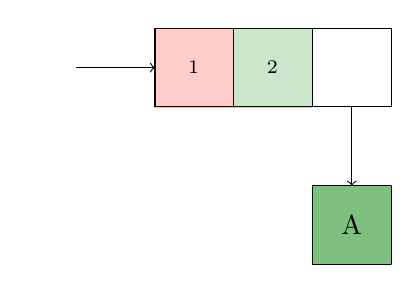
\begin{tikzpicture}[yscale=-1]
    \node at (0.5,0.5) {$\zooLoc$} ;
    \draw [->] (1,0.5) -- ++(1,0) ;
    \draw (2,0) grid ++(3,1) ;
    \draw [fill=red, opacity=0.2] (2,0) rectangle ++(1,1) ;
    \node at (2.5,0.5) {$\zooVal_1$} ;
    \draw [fill=Green, opacity=0.2] (3,0) rectangle ++(1,1) ;
    \node at (3.5,0.5) {$\zooVal_2$} ;
    \node at (4.5,0.5) {$\mcas$} ;
    \draw [->] (4.5,1) -- ++(0,1) ;
    \draw (4,2) grid ++(1,1) ;
    \draw [fill=Green, opacity=0.5] (4,2) rectangle ++(1,1) ;
    \node at (4.5,2.5) {A} ;
  \end{tikzpicture}}
  \caption{Successful MCAS}
  \label{fig:loc_representation_1}
  \end{subfigure}
\hfill
\begin{subfigure}{.3\textwidth}
  \centering
  \[
    \zooLoc \iPointstoTwo \zooVal_1
  \]
  \scalebox{.8}{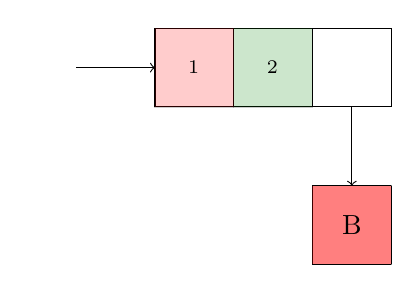
\begin{tikzpicture}[yscale=-1]
    \node at (0.5,0.5) {$\zooLoc$} ;
    \draw [->] (1,0.5) -- ++(1,0) ;
    \draw (2,0) grid ++(3,1) ;
    \draw [fill=red, opacity=0.2] (2,0) rectangle ++(1,1) ;
    \node at (2.5,0.5) {$\zooVal_1$} ;
    \draw [fill=Green, opacity=0.2] (3,0) rectangle ++(1,1) ;
    \node at (3.5,0.5) {$\zooVal_2$} ;
    \node at (4.5,0.5) {$\mcas$} ;
    \draw [->] (4.5,1) -- ++(0,1) ;
    \draw (4,2) grid ++(1,1) ;
    \draw [fill=red, opacity=0.5] (4,2) rectangle ++(1,1) ;
    \node at (4.5,2.5) {B} ;
  \end{tikzpicture}}
  \caption{Failed MCAS}
  \label{fig:loc_representation_2}
\end{subfigure}
\hfill
\begin{subfigure}{.38\textwidth}
  \centering
  \[
    \zooLoc \iPointstoTwo \zooVal_1
  \]
  \scalebox{.8}{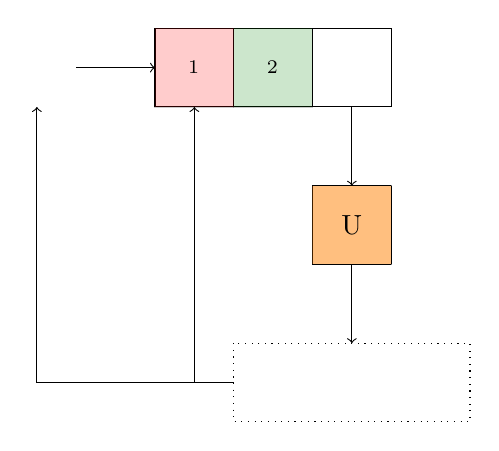
\begin{tikzpicture}[yscale=-1]
    \node at (0.5,0.5) {$\zooLoc$} ;
    \draw [->] (1,0.5) -- ++(1,0) ;
    \draw (2,0) grid ++(3,1) ;
    \draw [fill=red, opacity=0.2] (2,0) rectangle ++(1,1) ;
    \node at (2.5,0.5) {$\zooVal_1$} ;
    \draw [fill=Green, opacity=0.2] (3,0) rectangle ++(1,1) ;
    \node at (3.5,0.5) {$\zooVal_2$} ;
    \node at (4.5,0.5) {$\mcas$} ;
    \draw [->] (4.5,1) -- ++(0,1) ;
    \draw (4,2) grid ++(1,1) ;
    \draw [fill=orange, opacity=0.5] (4,2) rectangle ++(1,1) ;
    \node at (4.5,2.5) {U} ;
    \draw [->] (4.5,3) -- ++(0,1) ;
    \draw [dotted] (3,4) rectangle ++(3,1) ;
    \draw [->] (3,4.5) -| (0.5,1) ;
    \draw [->] (3,4.5) -| (2.5,1) ;
  \end{tikzpicture}}
  \caption{Undetermined MCAS}
  \label{fig:loc_representation_3}
\end{subfigure}
\caption{Representation of locations}
\label{fig:loc_representation}
\end{figure}


\paragraph{Representation of locations.}

An MCAS location (\ocamlinline{'a loc}) is represented as an atomic reference to a (mutable) \emph{descriptor} (\ocamlinline{'a state}), as shown in \cref{fig:loc_representation}.
A descriptor contains two values, one of which corresponds to the logical content of the location, and the MCAS operation it belongs to; this MCAS operation is the last to have \emph{locked} the location by writing the descriptor in question.
Crucially, each descriptor is unique and belongs to only one MCAS.

An MCAS operation (\ocamlinline{'a casn}) is represented as an atomic reference to a \emph{status} (\ocamlinline{'a status}).
When the MCAS has finished, its status is either \ocamlinline{After}, meaning it succeeded, or \ocamlinline{Before}, meaning it failed.
While the MCAS is still ongoing, its status is \ocamlinline{Undetermined}.
To make the algorithm lock-free, other operations have to be able to help the MCAS finish; therefore, an \ocamlinline{Undetermined} status links back to the target locations and the corresponding descriptors, resulting in a cyclic structure.

\def\myfigure#1#2{
  \begin{subfigure}{.45\textwidth}
    \centering
    \onlySet{#1}
    \scalebox{.5}{\begin{tikzpicture}[yscale=-1]
      \node at (0.5,0.5) {$\zooLoc_1$} ;
      
      \draw (2,0) grid ++(3,1) ;
      \draw [value_after] (2,0) rectangle ++(1,1) ;
      \node at (2.5,0.5) {1} ;
      \draw [value_after] (3,0) rectangle ++(1,1) ;
      \node at (3.5,0.5) {1} ;
      \node at (4.5,0.5) {$\mcas_1$} ;
      \draw [->] (4.5,0) -- ++(0,-1) ;
      \draw (4,-2) grid ++(1,1) ;
      \draw [state_after] (4,-2) rectangle ++(1,1) ;
      \node at (4.5,-1.5) {A} ;
      
      \node at (7.5,0.5) {$\zooLoc_2$} ;
      
      \draw (9,0) grid ++(3,1) ;
      \draw [value_after] (9,0) rectangle ++(1,1) ;
      \node at (9.5,0.5) {3} ;
      \draw [value_after] (10,0) rectangle ++(1,1) ;
      \node at (10.5,0.5) {3} ;
      \node at (11.5,0.5) {$\mcas_2$} ;
      \draw [->] (11.5,0) -- ++(0,-1) ;
      \draw (11,-2) grid ++(1,1) ;
      \draw [state_after] (11,-2) rectangle ++(1,1) ;
      \node at (11.5,-1.5) {A} ;
      
      \draw (2,2) grid ++(3,1) ;
      \only<1-4>{
        \draw [value_before] (2,2) rectangle ++(1,1) ;
        \node at (2.5,2.5) {1} ;
      }
      \only<5>{
        \draw [value_after] (2,2) rectangle ++(1,1) ;
        \node at (2.5,2.5) {2} ;
      }
      \only<1-5>{
        \draw [value_after] (3,2) rectangle ++(1,1) ;
        \node at (3.5,2.5) {2} ;
      }
      \node at (4.5,2.5) {$\mcas$} ;
      
      \draw (9,2) grid ++(3,1) ;
      \only<1-4>{
        \draw [value_before] (9,2) rectangle ++(1,1) ;
        \node at (9.5,2.5) {3} ;
      }
      \only<5>{
        \draw [value_after] (9,2) rectangle ++(1,1) ;
        \node at (9.5,2.5) {2} ;
      }
      \only<1-5>{
        \draw [value_after] (10,2) rectangle ++(1,1) ;
        \node at (10.5,2.5) {2} ;
      }
      \node at (11.5,2.5) {$\mcas$} ;
      
      \only<1-3>{
        \draw [state_undetermined] (7,4) rectangle ++(1,1) ;
        \node at (7.5,4.5) {U} ;
      }
      \only<4-5>{
        \draw [state_after] (7,4) rectangle ++(1,1) ;
        \node at (7.5,4.5) {A} ;
      }
      
      \draw [->] (4.5,3) |- (7,4.5) ;
      \draw [->] (11.5,3) |- (8,4.5) ;
      
      \only<1>{
        \draw [->] (1,0.5) -- ++(1,0) ;
      }
      \only<2>{
        \draw [->, orange] (0.5,1) |- (2,2.5) ;
      }
      \only<3-5>{
        \draw [->] (0.5,1) |- (2,2.5) ;
      }
      
      \only<1-2>{
        \draw [->] (8,0.5) -- ++(1,0) ;
      }
      \only<3>{
        \draw [->, orange] (7.5,1) |- (9,2.5) ;
      }
      \only<4-5>{
        \draw [->] (7.5,1) |- (9,2.5) ;
      }
    \end{tikzpicture}}
    \caption{#2}
    \label{fig:mcas_success_#1}
  \end{subfigure}
}

\begin{figure}
\centering
\myfigure{1}{Initial configuration}
\hfill
\myfigure{2}{Lock $\zooLoc_1$}
\par\bigskip
\myfigure{3}{Lock $\zooLoc_2$}
\hfill
\myfigure{4}{Signal state}
\par\bigskip
\myfigure{5}{Clean stale values}
\hfill
\strut
\caption{MCAS: Successful execution}
\label{fig:mcas_success}
\end{figure}

\def\myfigure#1#2{
  \begin{subfigure}{.45\textwidth}
    \centering
    \onlySet{#1}
    \scalebox{.5}{\begin{tikzpicture}[yscale=-1]
      \node at (0.5,0.5) {$\zooLoc_1$} ;

      \draw (2,0) grid ++(3,1) ;
      \draw [value_after] (2,0) rectangle ++(1,1) ;
      \node at (2.5,0.5) {1} ;
      \draw [value_after] (3,0) rectangle ++(1,1) ;
      \node at (3.5,0.5) {1} ;
      \node at (4.5,0.5) {$\mcas_1$} ;
      \draw [->] (4.5,0) -- ++(0,-1) ;
      \draw (4,-2) grid ++(1,1) ;
      \draw [state_after] (4,-2) rectangle ++(1,1) ;
      \node at (4.5,-1.5) {A} ;

      \node at (7.5,0.5) {$\zooLoc_2$} ;

      \draw (9,0) grid ++(3,1) ;
      \draw [value_after] (9,0) rectangle ++(1,1) ;
      \node at (9.5,0.5) {3} ;
      \draw [value_after] (10,0) rectangle ++(1,1) ;
      \node at (10.5,0.5) {3} ;
      \node at (11.5,0.5) {$\mcas_2$} ;
      \draw [->] (11.5,0) -- ++(0,-1) ;
      \draw (11,-2) grid ++(1,1) ;
      \draw [state_after] (11,-2) rectangle ++(1,1) ;
      \node at (11.5,-1.5) {A} ;

      \draw (2,2) grid ++(3,1) ;
      \draw [value_before] (2,2) rectangle ++(1,1) ;
      \node at (2.5,2.5) {1} ;
      \only<-2>{
        \draw [value_after] (3,2) rectangle ++(1,1) ;
        \node at (3.5,2.5) {2} ;
      }
      \only<3>{
        \draw [value_before] (3,2) rectangle ++(1,1) ;
        \node at (3.5,2.5) {1} ;
      }
      \node at (4.5,2.5) {$\mcas$} ;

      \draw (9,2) grid ++(3,1) ;
      \draw [value_before] (9,2) rectangle ++(1,1) ;
      \node at (9.5,2.5) {0} ;
      \only<-2>{
        \draw [value_after] (10,2) rectangle ++(1,1) ;
        \node at (10.5,2.5) {2} ;
      }
      \only<3>{
        \draw [value_before] (10,2) rectangle ++(1,1) ;
        \node at (10.5,2.5) {0} ;
      }
      \node at (11.5,2.5) {$\mcas$} ;

      \only<1>{
        \draw [state_undetermined] (7,4) rectangle ++(1,1) ;
        \node at (7.5,4.5) {U} ;
      }
      \only<2->{
        \draw [state_before] (7,4) rectangle ++(1,1) ;
        \node at (7.5,4.5) {B} ;
      }

      \draw [->] (4.5,3) |- (7,4.5) ;
      \draw [->] (11.5,3) |- (8,4.5) ;

      \only<1>{
        \draw [->, orange] (0.5,1) |- (2,2.5) ;
      }
      \only<2->{
        \draw [->] (0.5,1) |- (2,2.5) ;
      }

      \draw [->] (8,0.5) -- ++(1,0) ;
    \end{tikzpicture}}
    \caption{#2}
    \label{fig:mcas_failure_#1}
  \end{subfigure}
}

\begin{figure}
\centering
\myfigure{1}{Same configuration as \cref{fig:mcas_success_2} except the expected value for $\zooLoc_2$ (0) does not match the current value (3)}
\hfill
\myfigure{2}{Signal state}
\par\bigskip
\myfigure{3}{Clean stale values}
\hfill
\strut
\caption{MCAS: Failing execution}
\label{fig:mcas_failure}
\end{figure}


\paragraph{Locking.}

Comparatively to previous implementations like that of \citet{DBLP:conf/wdag/HarrisFP02}, this MCAS algorithm is simpler: it includes a locking phase but no unlocking phase.
On the other hand, there is an extra indirection for reads.

\Cref{fig:mcas_success} shows a successful execution of an MCAS operation.
Initially, the status is \ocamlinline{Undetermined}.
For each target location, the operation first checks that the current value is as expected and then attempts to atomically install its descriptor (\cref{fig:mcas_success_2,fig:mcas_success_3}), thereby ``locking'' the location.
If the locking phase succeeds, the operation then atomically updates its status to \ocamlinline{After} (\cref{fig:mcas_success_4}), which corresponds to the point when locations are logically modified.
Additionally, contrary to the original implementation, cleaning up is required to allow stale values to be garbage-collected (\cref{fig:mcas_success_5}).

\Cref{fig:mcas_failure} shows a failing execution of an MCAS operation.
If the operation finds an unexpected value during the locking phase, it atomically updates its status to \ocamlinline{Before} (\cref{fig:mcas_failure_2}) and cleans up stale values (\cref{fig:mcas_failure_3}).

\paragraph{Helping.}

So far, we only considered uncontended executions; in reality, one location may be targeted by concurrent \c{get} and \c{cas} operations.
Basically, everything happens just as before except operations help one another: if an operation encounters a descriptor whose MCAS operation is still in progress, it helps that MCAS operation to finish first.

\paragraph{Read-only operations}

When a location is read during a transaction, the generated MCAS operation includes a read-only CAS whose expected and desired value are the same; the intended behavior of this CAS is to only \emph{assert} that the location has not changed after the read.
As we have seen in the implementation, however, every location has to be locked for the MCAS to succeed.
This means two things: (1) CAS operations targeting the same location can only execute \emph{sequentially}; (2) CAS operations, even those that do not change the logical content of a location, cause \emph{contention} as after the operation only the cache of the writer will have a valid copy of the location.
This makes read-only CASes inefficient and unscalable.

To address this issue, we extended the algorithm to allow \emph{read-only} CMP operations to be expressed directly.
For example, the two transactions of \cref{sec:implementation_optimistic_approach} would generate the following operations:

\smallskip
\begin{minipage}[t]{.45\textwidth}
\begin{ocamlcode}
CMP (a, 10)
CMP (b, 52)
CAS (x, 0, 42)
\end{ocamlcode}
\end{minipage}
\hfill
\begin{minipage}[t]{.45\textwidth}
\begin{ocamlcode}
CMP (a, 10)
CMP (b, 52)
CAS (y, 0, 62)
\end{ocamlcode}
\end{minipage}
\smallskip

The idea is the following: at the start, we read the descriptors of read-only locations; at the end, after all other locations have been locked, we check that read-only locations have not changed before finishing the MCAS operation.
Crucially, CMP operations do \emph{not} write into memory, allowing them to run in parallel.

There is one drawback, however.
This new algorithm is \emph{obstruction-free} but not \emph{lock-free} like the original one.
In particular, two MCASes may cancel each other indefinitely.
To get the best of both worlds, \Kcas first attempts the MCAS operations in obstruction-free mode (CAS and CMP) and switches to lock-free mode (CAS only) after a number of failed attempts; the resulting algorithm is \emph{lock-free}.

\clearpage
\section{Verified Multi-Word Compare-and-Set Algorithm}
\label{sec:verification}

The correctness of \Kcas transactions relies on that of the underlying MCAS algorithm (see \cref{sec:implementation_mcas}), whose implementation (\cref{fig:mcas_code_1,fig:mcas_code_2,fig:mcas_code_3}) is short but extremely subtle.
We verified the algorithm~\refLibTheoriesFile{zoo_mcas/mcas} using the \Zoo framework~\citep{DBLP:journals/pacmpl/AllainS26}, which provides (1) a translator from \OCaml to \Rocq and (2) a precise semantics for concurrent primitives (such as \ocamlinline{Atomic.compare_and_set}) and physical equality.
All our proofs are mechanized in the \Rocq proof assistant.

Note that \Zoo assumes a \emph{sequentially consistent} memory model whereas \OCamlFive has a \emph{relaxed} memory model~\citep{DBLP:conf/pldi/DolanSM18}.
We inherit the limitation and conjecture that this assumption does not invalidate our concurrent invariant, the core of the proof, and that it can be adapted to relaxed memory following the ``recipe'' of \citet{DBLP:journals/pacmpl/MevelJ21}.

\subsection{Specification}

\begin{figure}
\begin{mathpar}
    \iSpec[
      lab=make-spec
    ]{
      \iTrue
    }{
      \c{make}\ \zooVal
    }[
      \zooLoc
    ]{
      \locInv\ \zooLoc\ \iIname \iSep \\
      \zooLoc \iPointstoTwo \zooVal
    }
  \and
    \iAspec[
      lab=get-spec,
      mask=\iIname
    ]{
      \locInv\ \zooLoc\ \iIname
    }[
      \zooVal
    ]{
      \zooLoc \iPointstoTwo \zooVal
    }{
      \c{get}\ \zooLoc
    }{
      \zooLoc \iPointstoTwo \zooVal
    }[
      \zooValTwo
    ]{
      \zooVal \similar \zooValTwo
    }
  \and
    \iAspec[
      lab=cas-spec,
      mask=\iIname
    ]{
      \iBigSep_{\zooLoc \in \zooLoc{}s}
        \locInv\ \zooLoc\ \iIname
    }[
      \zooVals
    ]{
      \iBigSep_{\zooLoc, \zooVal \in \zooLoc{}s, \zooVals}
        \zooLoc \iPointstoTwo \zooVal
    }{
      \c{cas}\ \zooLoc{}s\ \v{befores}\ \v{afters}
    }[
      \zooBool
    ]{
      \myif{
        \zooBool
      }{
        \begin{inbox}
          \zooVals \similar \v{befores} \iSep \\
          \iBigSep_{\zooLoc, \zooVal \in \zooLoc{}s, \v{afters}}
            \zooLoc \iPointstoTwo \zooVal
        \end{inbox}
      }{
        \begin{inbox}
          \Exists i\ \zooVal\ \v{before}. \\
          \mapLookup{\zooVals}{i} = \Some{\zooVal} \iSep \\
          \mapLookup{\v{befores}}{i} = \Some{\v{before}} \iSep \\
          \zooVal \nonsimilar \v{before} \iSep \\
          \iBigSep_{\zooLoc, \zooVal \in \zooLoc{}s, \zooVals}
            \zooLoc \iPointstoTwo \zooVal
        \end{inbox}
      }
    }[
      \v{res}
    ]{
      \v{res} = \zooBool
    }
\end{mathpar}
\caption{MCAS: Specification}
\label{fig:mcas_spec}
\end{figure}


The specification of MCAS is given in \cref{fig:mcas_spec}.
The persistent assertion $\locInv\ \zooLoc\ \iIname$ represents the knowledge that \zooLoc is a valid MCAS location.
The exclusive assertion $\zooLoc \iPointstoTwo \zooVal$ represents the ownership of location \zooLoc and the knowledge that it contains value \zooVal.
$\c{make}\ \zooVal$ creates a new location initialized with \zooVal.
$\c{get}\ \zooLoc$ atomically reads the content of \zooLoc.
$\c{cas}\ \zooLoc{}s\ \v{befores}\ \v{afters}$ performs an MCAS operation on locations $\zooLoc{}s$ with expected values \v{befores} and desired values \v{afters}; on success, it atomically updates $\zooLoc{}s$ from \v{befores} to \v{afters}; on failure, it must have observed a location whose value was different than expected.

\subsection{Linearization}

\paragraph{External linearization.}

As explained in \cref{sec:implementation_mcas}, an MCAS operation may be helped and in fact linearized by another MCAS.
Consequently, the linearization point of both \c{get} and \c{cas} may be external.
In fact, a helper may linearize many operations at once, including the original MCAS and other helpers.
Also, a helper may linearize a helped MCAS while helping yet another MCAS.

\paragraph{Future-dependent linearization.}

When two operations helping an MCAS detect an unexpected value, they both attempt to atomically update its status to B.
The question is: which of them linearizes the MCAS operation (and other helpers) at the point when it observes an unexpected value?
The answer is: the one which ``wins'' the update.
Consequently, the linearization point of \c{cas} may also be future-dependent.

\subsection{Challenges}

% + prophecy variables (Zoo.proph, Zoo.resolve, Zoo.resolve_with)
% + ghost identifiers (Zoo.id)

The implementation is fairly short (one hundred lines of code) but extremely subtle.
We outline the main challenges.

\paragraph{Mutually recursive invariants.}

Due to the cyclic structure of ongoing MCASes (see \cref{fig:loc_representation_3}), the definitions of the location invariant (\locInv) and the MCAS invariant are mutually recursive.
Thankfully, \Iris provides a way to define such fixpoints.

Another difficulty comes from the fact that the creation of a location involves a dummy MCAS operation whose invariant has to be initialized at the same time as the location's.
We had to introduce a way to break the cycle.

\paragraph{Logical state.}

The verification involves a monotonic logical status that is not determined by the physical status: the physical U status is divided into indexed logical U status indicating the progress made by the MCAS operation.

\paragraph{External linearization.}

To handle external linearization of an MCAS operation and its helpers by a helper, their atomic updates%
\footnote{
In \Iris, an \emph{atomic update} is a resource that materializes a linearization point.
\Citet{DBLP:journals/pacmpl/MulderK23} provide a good description.
}
are stored into the MCAS invariant.
At the linearization point, the winning helper triggers all the atomic updates and puts them back into the invariant to be retrieved later by their respective owner.

\paragraph{Global prophecy variable.}

To handle future-dependent linearization, we predict both the winner and the outcome of an MCAS operation through a shared prophecy variable.
To distinguish the winner, we use the same trick as \citet{DBLP:journals/pacmpl/JungLPRTDJ20} in their proof of RCDSS: each MCAS participant is assigned a unique physical identifier (implemented using a prophecy variable) that is part of the prediction.

\paragraph{Local prophecy variable.}

For subtle reasons related to the semantics of physical equality~\citep{DBLP:journals/pacmpl/AllainS26}, we also need to introduce a local prophecy variable in \c{cas}.
Essentially, the problem is that we cannot predict the outcome of physical equality in advance just by looking at the values; in other words, equality in \Rocq does not imply physical equality in \OCaml.

% generative constructors

\paragraph{MCAS history.}

Another subtle point in the algorithm is the fact that a location cannot be locked more than once by a single MCAS operation.
While this is obvious when reading the code, it is not in the proof.
To enforce it logically, each location maintains a ghost history of distinct MCASes; all MCAS in this history are finished except the more recent one.

\clearpage
\section{Benchmarks}
\label{sec:benchmarks}

% compared with lock-based algorithms, principal advantage is composability rather than raw throughput

\clearpage
\section{Related Work}

\paragraph{Software transactional memory}

% other implementations
% + Haskell
% + Scala: ZIO
% + C++: cpp_stm_free

% \cite{DBLP:conf/podc/ShavitT95}

% \cite{DBLP:conf/ppopp/HarrisMPH05}
% \cite{DBLP:conf/flops/DiscoloHMJS06}
% \cite{DBLP:conf/haskell/LeYF16}

\paragraph{Multi-word compare-and-set}

% \cite{DBLP:conf/wdag/HarrisFP02}
% \cite{DBLP:conf/wdag/GuerraouiKMZ20}

We believe that our work is the first verification of the MCAS algorithm of \citet{DBLP:conf/wdag/GuerraouiKMZ20} and more generally the first foundational verification of an MCAS algorithm.
We are aware of one closely related line of work.
\Citet{DBLP:phd/ethos/Vafeiadis08} sketches a proof of the RDCSS and MCAS algorithms of \citet{DBLP:conf/wdag/HarrisFP02}.
However, \citet{DBLP:journals/pacmpl/JungLPRTDJ20} show that his proof of RDCSS is flawed and verify it in \Iris, using prophecy variables; they also verify both RDCSS and MCAS using \VeriFast~\citep{DBLP:conf/nfm/JacobsSPVPP11}.

\paragraph{Prophecy variables}

% \cite{DBLP:journals/pacmpl/JungLPRTDJ20}
% \cite{DBLP:phd/ethos/Vafeiadis08}
% \cite{DBLP:conf/osdi/Chang0STKZ23}

\clearpage
\input{conclusion}
\clearpage

% ---------------------------------------------------------

\hbadness=10000
\bibliography{main}

\end{document}
